\label{app:ks}
\section{Bayesian Generative Search}
\label{app-ks-sec:method}
Similar to~\citet{Lu18}, we reformulate the discrete optimization problem as a BO task over a latent representation space, which allows us to bypass both the need to select an initial set of active candidates~\cite{Duvenaud13} and to rely on heuristic methods for exploring new candidates~\cite{Malkomes16}. However, instead of learning a direct embedding, we implicitly encode composite kernels as output of a parameterized \emph{open-ended recurrent generator}. While~\citet{Lu18} focuses on learning a mapping between latent representations and kernel expressions, our method, \textsc{DTerGenS}, learns a mapping between the latent coordinates and the \emph{infinitely long} kernel expression generative trajectories. This main difference helps to avoid placing an explicit upper limit on the expression length, thus ensuring sufficient expressiveness of the candidate set. 

\begin{figure}
\centering
\begin{tikzpicture}
  \node[group2, minimum size=1cm] (g) {\textsc{Generator} $G$};
  \node[neuron, left=2em of g] (t) {$\theta$};
  \node[neuron, below=2em of g] (p) {$\pi$};
  \node[io, right=2em of g] (k) {$k$};
  \node[io, right=2em of k] (f) {$F_{\tau}(k)$};
  \draw[conn] (t) -- (g);
  \draw[conn] (p) -- (g);
  \draw[conn] (g) -- (k);
  \draw[conn] (k) -- (f);
  \draw [dashed,->] (f.south) to [out=-122,in=0] (p.east) node[below right=1.2em, rotate=8]{\ \ \ \ \ \ \ \textsc{PolicyUpdate}};
  \draw [dashed,->] (p.west) node[below left=0.5em, rotate=-10]{\textsc{BayesOpt}\ \ } to [out=-185,in=-80] (t.south);
\end{tikzpicture}
\caption{The generic workflow of \textsc{DTerGenS}. Given policy $\pi$, we employ BO to obtain generative weight candidate $\theta$ (Section~\ref{app-ks-subsec:theta}). Using the observed generative trajectory, we alternately update the policy distribution (Section~\ref{app-ks-subsec:pi}).}
\label{app-fig:workflow}
\end{figure}

The VAE decoder in~\cite{Lu18}, which sequentially generates the next operand and operator given the current expression, is pre-trained with the VAE encoder using randomly sampled kernel expressions. In contrast, our generator explicitly captures the \emph{sum-of-product} structure through a nested recursion procedure, thus is capable of generalizing the composition rules to create new expressions. To prevent the generation of infinitely long and computationally expensive expressions, we learn a stochastic early stopping policy, which determines the best performing stopping point on any generative trajectory. This method enables the exploration of arbitrarily complex expressions and is the first selection method that places no further structural restriction on the search space.

Both the generative parameters and the termination policy can be jointly optimized by exploiting their dynamic in the generative component. Fixing a termination policy, we devise a dynamic BO algorithm for optimizing generative parameters that is capable of adapting to the constant policy updates. Alternately, given each sample trajectory collected by the BO step, we devise an update algorithm for the policy distribution via modelling the dynamic between these two components. Together, these steps compose our main contribution, which is the \textsc{DTerGenS} algorithm for composite kernel selection. 

We demonstrate that \textsc{DTerGenS} is able to produce sophisticated kernel expressions, which significantly improve the predictive performance over state-of-the-art methods on multiple benchmarks. Our results show a wider range of structures being explored by \textsc{DTerGenS} and faster convergence compared to other methods. Finally, we show that \textsc{DTerGenS} is also able to recover known well-performing kernels on artificially designed predictive tasks.

\subsection{Reformulating Kernel Selection}
\label{app-ks-subsec:reformulation}
Directly optimizing over the discrete domain of kernel expressions as suggested by Definition~\ref{c3-def:ksproblem} is challenging. To work around this, we model $k$ as the output of a generative process $G(\theta, \pi)$ conditioned on $\theta$ and $\pi$, which controls the termination of $G$. The designs of $G$ and $\pi$ are given in Section~\ref{app-ks-subsec:generator} and Section~\ref{app-ks-subsec:pi} respectively. We approximate the original kernel selection objective in Definition~\ref{c3-def:ksproblem} as:
\begin{eqnarray}
\underset{k \in \mathcal{K_C}}{\argmax} \ F_{\Omega}(k) &\simeq&  \underset{\theta \in \Theta, \pi \in \Pi}{\argmax} \ R_{\tau} (\theta, \pi) \ ,
\label{app-ks-prop:reformulation}
\end{eqnarray}
where $R_\tau$ is defined as the composite function $F_\tau \circ G$.

\noindent Our framework alternately optimizes each component $\pi$ and $\theta$ while fixing the other as constant. Explicitly, given a policy $\pi$, the generative parameter $\theta$ is optimized using an adapted BO algorithm that is formulated with the conditional policy distribution $p(\pi \mid \theta)$ (Section~\ref{app-ks-subsec:theta}). On the other hand, given the BO-sampled observations, the policy distribution $p(\pi \mid \theta)$ can be updated via MLE (Section~\ref{app-ks-subsec:pi}). The outline of this workflow is illustrated in Fig.~\ref{c3-fig:workflow}. To lay the groundwork for our algorithmic development, we will first discuss the design of our kernel generator $G(\theta, \pi)$ in Section~\ref{app-ks-subsec:generator}.

\subsection{Open-ended Kernel Generator}
\label{app-ks-subsec:generator} 
A composite kernel expression, written as a sum-of-products over base kernel units in Eq.~\eqref{c3-eq:general}, naturally manifests as a tree with (1)~a primary linear chain; and (2)~several secondary linear branches that are connected to the primary chain. The secondary branches denote different products of base kernel units, whereas the primary chain denotes the summation over them. To generate such structures, we construct $G$ by composing two nested recurrent units, which are described below. Fig.~\ref{app-ks-fig:generator} further visualizes the blueprint of this generator architecture.
\subsubsection{Generator Overview}
Our generator architecture comprises of a primary unit and a secondary unit, which respectively generate the primary chain and the secondary branches. Each unit composes of a recurrent neural network (RNN) and a termination policy, which predicts a stopping signal given the hidden state of the neural network. Every recurring step of the primary unit initiates a new secondary branch and computes an initial hidden state for the secondary RNN. On the other hand, every recurring step of the secondary unit generates a new base kernel unit on the current branch. Each unit will recur until its respective policy outputs a stopping signal given the respective current hidden state. When the primary unit terminates, we output a tree structure corresponding to a composite kernel. We give the mechanism of each component below.
\begin{figure}[t]
\centering
\begin{tikzpicture}
  \node[io] (x0) {$h_0$};
  \node[neuron,right=of x0] (x1)
  {$h_{1}$};
  \node[neuron,right=4em of x1] (dot)
  {$\ldots$}; 
  \node[neuron,right=4em of dot] (xM)
  {$h_{m}$};
  
  \node[neuron,below=1.5em of x1] (x1_0)
  {$h_{1,0}$};
  \node[neuron,below=1em of x1_0] (x1_1)
  {$h_{1,1}$};
  \node[neuron,below=1em of x1_1] (dot2)
  {$\ldots$};
  \node[right=4.5em of dot2] (dot3)
  {$\ldots$}; 
  \node[io,right=4em of x1_1] (o1_1)
  {$k_{1,1}$};
  \node[neuron,below=1em of dot2] (x1_N)
  {$h_{1, n_1}$};
  \node[io,right=4em of x1_N] (o1_N)
  {$k_{1, n_1}$};
  
  \node[neuron,below=1.5em of xM] (xM_0)
  {$h_{m,0}$};
  \node[neuron,below=1em of xM_0] (xM_1)
  {$h_{m,1}$};
  \node[neuron,below=1em of xM_1] (dot4)
  {$\ldots$};
  \node[right=4.5em of dot4] (dot5)
  {$\ldots$}; 
  \node[io,right=4em of xM_1] (oM_1)
  {$k_{m,1}$};
  \node[neuron,below=1em of dot4] (xM_N)
  {$h_{m, n_1}$};
  \node[io,right=4em of xM_N] (oM_N)
  {$k_{m, n_m}$};
  
  \node[left=1.5em of dot2] (gs)
  {$\mathcal{U}_s \equiv (G_s, \pi_s)$};
  \node[above=1em of dot] (gp)
  {$\mathcal{U}_p \equiv (G_p, \pi_p)$};
  \node[group,fit={(x1) (dot) (xM)}] (gr1) {};
  \node[group,fit={(x1_1) (dot2) (x1_N)}] (gr2) {};
  \node[group,fit={(xM_1) (dot4) (xM_N)}] (gr3) {};
  \draw[conn] (x0) -- (x1);
  \draw[conn] (x1) -- (dot);
  \draw[conn] (dot) -- (xM);
  
  \draw[conn] (x1) -- (x1_0);
  \draw[conn] (x1_0) -- (x1_1);
  \draw[conn] (x1_1) -- (dot2);
  \draw[conn] (dot2) -- (x1_N);
  \draw[conn] (x1_1) -- (o1_1);
  \draw[conn] (x1_N) -- (o1_N);
  
  \draw[conn] (xM) -- (xM_0);
  \draw[conn] (xM_0) -- (xM_1);
  \draw[conn] (xM_1) -- (dot4);
  \draw[conn] (dot4) -- (xM_N);
  \draw[conn] (xM_1) -- (oM_1);
  \draw[conn] (xM_N) -- (oM_N);
\end{tikzpicture}
\caption{Schematic of the kernel generator with nested units $\mathcal{U}_p$ and $\mathcal{U}_s$. Each component recursively computes its next hidden state and emission output using respective recurrent neural network $G_s$ and $G_p$. The termination probability at each generative step is determined by policies $\pi_p$ and $\pi_s$. The final candidate kernel expression is composed using Eq.~\eqref{c3-eq:general}.}
\label{app-ks-fig:generator}
\end{figure}
\subsubsection{Primary Unit}
The primary unit $\mathcal{U}_p: \mathbb{R}^{d_p} \rightarrow \mathcal{K_C}$ is given by the RNN $G_p$ and the policy $\pi_p: \mathcal{K_C} \rightarrow \mathbb{R}$. $G_p$ has hidden dimension $d_p$ and emits an initial hidden state for $G_s$. Given an arbitrary initial hidden state $h_0 \in \mathbb{R}^{h_p}$, $G_p$ performs the following at any generative step $t \geq 0$:
\begin{itemize}
\item If $t=0$, initialize candidate kernel expression $\bar{k} = 0$ (i.e., a constant function).
\item Generate the next hidden state and the current emission output: $(h_{t+1}, h_{t,0}) \leftarrow G_p(h_t; \theta_t)$. 
\item Generate and append the $t^{\text{th}}$ secondary branch to the current expression: $\bar{k} \leftarrow \bar{k} + \mathcal{U}_s(h_{t,0}; \theta_s, \pi_s)$.
\item Query termination probability with the current intermediate expression: $\alpha \leftarrow \pi_p(\bar{k})$. 
\item With probability $\alpha$, end the generative procedure and return $\bar{k}$ as a terminal expression. 
\item With probability $1 - \alpha$, set $t \leftarrow t+1$ and repeat the procedure.
\end{itemize}

\subsubsection{Secondary Unit}
The secondary unit $\mathcal{U}_s: \mathbb{R}^{d_s} \rightarrow \mathcal{K_C}$ is given by the RNN $G_s$ and the policy $\pi_s: \mathcal{K_C} \rightarrow \mathbb{R}$. $G_s$ has hidden dimension $d_s$ and emits one-hot representations of the base kernel units in $\mathcal{K_B}$. Given an initial hidden state $h \in \mathbb{R}^{d_s}$ output by $G_p$, $\mathcal{U}_s$ generates a corresponding product of base kernel units. Given an initial hidden state $h_{t,0}$ produced by $G_p$ at time $t$, $G_s$ then performs the following at any inner loop generative step $t' \geq 0$:
\begin{itemize}
    \item If $t'=0$, initialize the inner loop kernel expression $\bar{k}_t = 1$ (i.e., a constant function).
    \item Generate the next hidden state and emit the current base kernel: $(h_{t, t'+1}, k_{t, t'})~\leftarrow~G_s(h_{t, t'}; \theta_s)$.
    \item Extend current expression via multiplication: $\bar{k}_t = \bar{k}_t \times k_{t, t'}$.
    \item Query the termination probability $\beta \leftarrow \pi_s(\bar{k} + \bar{k}_t)$.
    \item With probability $\beta$, end the generative procedure for the current branch and return $\bar{k}_t$.
    \item With probability $1 - \beta$, set $t' \leftarrow t' + 1$ and repeat the procedure.
\end{itemize}
\subsubsection{Termination Policy}
Let $\tau = \{\mathbf{x}_1, \mathbf{x}_2 \ldots \mathbf{x}_n\}$ denote the set of training inputs specified by the learning instance $\Omega$, as introduced in Definition~\ref{c3-def:ksproblem}. The termination policies $\pi_p$ and $\pi_s$, respectively parameterized by the neural networks $\gamma_p$ and $\gamma_s$, are given as follows:
\begin{eqnarray}
\pi_p(k; \gamma_p, \tau) &\triangleq& \sigma\left(\sum_{i,j\in[n]}\gamma_p(\mathbf{x}_i)\cdot\gamma_p(\mathbf{x}_j)\cdot k(\mathbf{x}_i,\mathbf{x}_j)\right)\nonumber \ , \\ 
\text{and} \quad \pi_s(k; \gamma_s, \tau) &\triangleq& \sigma\left(\sum_{i,j\in[n]}\gamma_s(\mathbf{x}_i)\cdot\gamma_s(\mathbf{x}_j)\cdot k(\mathbf{x}_i,\mathbf{x}_j)\right) \ ,
\end{eqnarray} 
where $\sigma(t) \triangleq 1/(1 + \mathrm{exp}(-t))$ denotes the sigmoid activation function. This data-driven parameterization serves to model the task-specific termination rules conditioned on observation task data, which implies that different expression lengths are required for different tasks. We further model the interaction between generative weights $\theta$ and termination policies $\pi$ using the conditional distributions $p(\gamma_s \mid \theta)$ and $p(\gamma_p \mid \theta)$, which in turn are used to construct a kernel function (that models the covariance between composite kernels) of an adapted BO routine (Section~\ref{app-ks-subsec:theta}). This allows us to sample policies given a candidate generative weight and distills finite kernel expression from the potentially infinite trajectory. On the other hand, the adapted BO routine will collect the full trajectory of kernel generation per iteration (consisting of all intermediate expressions until the termination point). This is then used to optimize the above conditional distribution via minimizing a heuristic loss function, thus allowing us to alternately learn the dynamics between $\theta$ and $\pi$ (Section~\ref{app-ks-subsec:pi}).

\subsection{Generative Parameter Optimization}
\label{app-ks-subsec:theta}
% \begin{algorithm}[tb]
%   \caption{\textsc{DTerGenS} - Kernel Selection}
%   \label{alg.dtergens}
% \begin{algorithmic}[1]
%   \STATE {\bfseries Input:}  $\mathcal{F}_\Omega$, $n_{\mathrm{BO}}$, $\gamma = \{n_w, n_\epsilon, n_\ell, \lambda_p, \lambda_s\}$
%   \STATE $\mathcal{G} \leftarrow$ \textsc{CreateGenerator}
%   \STATE $\eta_p,\eta_s \leftarrow$ \textsc{InitializePolicy}
%   \FOR{$t=1$ {\bfseries to} $n_{\mathrm{BO}}$}
%   \STATE $\theta^t \leftarrow {\mathrm{argmax}}_\theta\ f_{\mathrm{acq}}(\theta)$
%   \STATE \textsc{Sample} $\pi_p \sim p(\pi_p \mid \theta^t_p)$
%   \STATE \textsc{Sample} $\pi_s \sim p(\pi_s \mid \theta^t_s)$
%   \STATE $\mathbf{k}_t \leftarrow \mathcal{G}(\theta^t, \pi_p, \pi_s)$
%   \STATE $\mathbf{k}^\ast \leftarrow \mathrm{argmax}_{\mathbf{k} \ \subseteq_{\mathcal{K}}\mathbf{k}_t} \ \mathcal{F}_\Omega(\mathbf{k})$
%   \STATE \textsc{PolicyUpdate}$(\mathbf{k}^\ast,\theta^t,\gamma)$
%   \STATE \textsc{BayesianUpdate}$\left(\theta^t, \mathcal{F}_\Omega(\theta^t), p(\pi_p|\theta^t_p),p(\pi_s|\theta^t_s)\right)$
%   \ENDFOR
% \end{algorithmic}
% \end{algorithm}

In this section, we detail our BO algorithm to optimize the generative weight $\theta$. Formally, fixing a policy distribution $\bar{\pi}$ whose parameterization $\bar{\gamma}$ follows the conditional distribution $\bar{p}(\gamma \mid \theta) \triangleq \bar{p}(\gamma_p \mid \theta)\bar{p}(\gamma_s \mid \theta)$, the partial objective can be rewritten as:
\begin{eqnarray}
\theta^\ast \ = \ \underset{\theta\in\Theta}{\argmax} \  g_{\bar{\pi}}(\theta) & \equiv & \underset{\theta \in \Theta}{\argmax} \ \mathbb{E}_{\gamma \sim \bar{p}}\left[ R_\tau(\theta, \pi(\gamma))\right] \ .
\end{eqnarray}
We then adopt the standard practice of BO~\cite{Snoek12} and impose a Gaussian Process (GP)~\cite{Rasmussen06} prior on the black-box function $g_{\bar{\pi}}$, i.e., $g_{\bar{\pi}} \sim \mathcal{GP}(\mu, k_{\mathrm{BO}})$ where $\mu$ and $k_{\mathrm{BO}}$ respectively denote its mean and covariance functions. The BO algorithm iteratively obtains the next best candidate $\theta$ by maximizing a surrogate acquisition function constructed from the posterior distribution of this GP. The black-box evaluation $g_\pi(\theta)$ is then used to update the GP posterior.

Note that in standard BO setting, the functional landscape is static, whereas in our formulation $\bar{\pi}$ is alternately optimized after every BO iteration, which results in a changing function $g_{\bar{\pi}}$. To account for this dynamic update of ${\bar{\pi}}$, we will therefore model the GP covariance using two components: (1)~an intrinsic kernel component that characterizes the feature distance between the generative weights $\theta_i$ and $\theta_j$; and (2)~an extrinsic kernel component that captures the divergence of their conditional policy distribution $p(\gamma \mid \theta_i)$ and $p(\gamma \mid \theta_j)$ given the current parameterization $\gamma_p$, $\gamma_s$. Explicitly, given candidates $\theta_i$ and $\theta_j$, the kernel distance between these candidates is given as:
\begin{eqnarray}
k_{\mathrm{BO}}(\theta_i, \theta_j) &\triangleq& k_{\textsc{Policy}}(\theta_i, \theta_j)\cdot k_{\textsc{Generator}}(\theta_i, \theta_j) \ ,
\end{eqnarray}
where $k_{\textsc{Generator}}$ is given by the standard squared exponential kernel and $k_{\textsc{Policy}}$ is given by the symmetric KL divergence between the policy distributions conditioned on $\theta_i$ and $\theta_j$ respectively:
\begin{eqnarray}
k_{\textsc{Policy}}(\theta_i, \theta_j) &\triangleq& \mathbb{KL}\Big(p(\gamma\mid\theta_i) \ \| \ p(\gamma \mid\theta_j)\Big)  \ .
\end{eqnarray}

\subsection{Optimizing Policy Distribution}
\label{app-ks-subsec:pi}
We use the same notation $\gamma$ to refer to both policy $\gamma_p$ and $\gamma_s$ in this section due to their symmetry. We first give our parameterization for the policy distribution $p(\gamma \mid \theta)$ using a standard Bayesian neural networks:
\begin{eqnarray}
p(\gamma \mid \theta) &\sim& \mathcal{N}(\gamma_p; \mu(\theta), \Sigma(\theta)) \ ,
\end{eqnarray}
where $\mu$ and $\Sigma$ are deep neural networks that respectively generate the mean and covariance of the distribution. This section then details an update iteration of $\mu$ and $\sigma$ given a new candidate weight $\theta$ (derived from maximizing the BO acquisition function) and its corresponding kernel expression $k = \sum_{t=1}^m\prod_{t'=1}^{n_t} k_{t, t'}$ where $k_{t, t'} \in \mathcal{K_B}$. Since the generative trajectory encoded by $\theta$ is infinite, there is no analytical method to compute its optimal set of stopping points. However, we can approximate the optimal stopping point in this trajectory by finding the best performing intermediate kernel expression on the observed finite trajectory. Explicitly, let $\mathcal{S} = \{\{\bar{m}, \bar{n}_1, \bar{n}_2 \dots \bar{n}_m\} \mid \bar{m} \leq m, \forall t \in [\bar{m}]: \ \bar{n}_t \leq n_t\}$ be the set of all possible intermediate sets of stopping points that precede $k$, we define the \emph{hindsight estimation} of $k$ as:

\begin{eqnarray}
k^\ast &=& \sum_{t=1}^{m^\ast}\prod_{t'=1}^{n^{\ast}_{t}} k_{t, t'}, \quad \text{where} \nonumber \\
\{m^\ast, n^\ast_1 \dots n^\ast_{m^{\ast}}\} &\triangleq& \underset{
 \{m', n'_1, \dots n'_m\} \in \mathcal{S}
}{\argmax} F_{\tau}\left(\sum_{t=1}^{m'}\prod_{t'=1}^{n'_{t}} k_{t, t'}\right) \ ,
\end{eqnarray}
and let $K^\ast_{\tau}$ denote the covariance matrix induced by $k^\ast$ on training inputs the ${\mathcal{D}}$ described in $\tau$. We argue that high-performing kernels likely produce covariance matrices that are similar to $K^\ast_{\tau}$ , which motivates the following loss function with respect to current candidate weight $\theta$ :
\begin{eqnarray}
\mathcal{L}_\theta(\mu, \sigma) &=& \mathbb{E}_{\gamma\sim \mathcal{N}(\mu(\theta), \sigma(\theta))}\Big[ \left\langle{G}(\theta, \pi(\gamma)),k^\ast\right\rangle_{\tau}\Big] \nonumber \\
&\simeq& \frac{1}{r_{\gamma}}\sum_{i=1}^{r_{\gamma}} \left\langle{G}(\theta, \pi(\gamma_i)),k^\ast\right\rangle_{\tau}
\end{eqnarray}
where $r_\gamma$ denotes the number of $\gamma$ samples drawn from the conditional distribution; $\pi(\gamma_i)$ denotes the termination policy parameterized by $\gamma_i$ drawn from the conditional policy distribution; $G(\theta, \pi(\gamma_i))$ denotes the kernel expression generated by $G$ with weight $\theta$ and policy $\pi(\gamma_i))$; and $\langle k, k'\rangle_{\tau} \triangleq \|K_{\tau}-K'_{\tau}\|_{\mathrm{Fro}}$ denotes the Frobenius norm of the difference between the covariance matrices induced by kernel functions $k$ and $k'$. This loss function, however, does not have an analytical gradient with respect to $\mu$ and $\sigma$ as it requires simulation to compute. To optimize for $\mu$ and $\sigma$, we first employ the random gradient estimation technique~\cite{nesterov17}, which approximates gradient at a point by evaluating the expected gradient of its $\upsilon$-Gaussian smoothing. In particular, we derive our randomized gradient estimation for $\mu$ as follows:
\begin{eqnarray}
\nabla_{\mu} \mathcal{L}_\theta(\mu, \sigma) &\simeq& \nabla_\mu \  \mathbb{E}_{\upsilon\sim\mathcal{N}(0, \mathbf{I})}\left[\ell_\theta(\mu + \upsilon, \sigma)\right] \nonumber \\
&=& \mathbb{E}_{\upsilon\sim\mathcal{N}(0, \mathbf{I})}\left[\ell_\theta(\mu + \upsilon, \sigma)\upsilon\right] \nonumber \\
&\simeq& \frac{1}{r_\upsilon} \sum_{j=1}^{r_\upsilon} \ell_\theta(\mu + \upsilon_j, \sigma)\upsilon_j \nonumber
\\ 
&\simeq& \frac{1}{r_\gamma r_\upsilon} \sum_{i=1}^{r_\gamma}\sum_{j=1}^{r_\upsilon} \left\langle G(\theta, \pi(\mu_i + \upsilon_j, \sigma_i), k^{\ast} \right\rangle_{\tau} \ ,
\end{eqnarray}
where $r_\upsilon$ denotes the number of $\upsilon$ samples drawn from the standard Gaussian distribution $\mathcal{N}(0, \mathbf{I})$ and we have rewritten $\pi(\gamma_i) = \pi(\mu_i, \sigma_i)$ to clearly show the perturbed component $\mu_i$ in the estimation. Similarly, the gradient estimation for $\sigma$ is given as:
\begin{eqnarray}
\nabla_{\sigma} \mathcal{L}_\theta(\mu, \sigma) &\simeq& \frac{1}{r_\gamma r_\upsilon} \sum_{i=1}^{r_\gamma}\sum_{j=1}^{r_\upsilon} \left\langle G(\theta, \pi(\mu_i, \sigma_i + \upsilon_j), k^{\ast} \right\rangle_{\tau} \ .
\end{eqnarray}
These estimations allow us to update $\mu$ and $\sigma$ via the gradient descent algorithm, which complete the specification of our policy update. 

\section{Experiments}
\label{app-ks-sec:exp}
This section evaluates and reports the empirical performance of our kernel selection framework $\textsc{DTerGenS}$ on a synthetic kernel recovery task and kernel selection for regression on three real-world datasets:
\begin{itemize}
\item The DIABETES dataset~\cite{UCI_diabetes_data} contains 442 diabetes patient records (i.e., inputs) with 10 variables: age, sex, body mass index, average blood pressure and six blood serum measurements. The target output variable is a quantitative measure of disease progression one year after baseline.
\item The MAUNA LOA dataset~\cite{mauna_loa_data} measures monthly average $\mathrm{CO}_2$ concentration (in ppvm) of air samples at the Mauna Loa Observatory over 42 years (i.e., 504 observations in total).
\item The PROTEIN dataset~\cite{UCI_protein_data} features 45730 observations of protein tertiary structures, each records 9 physicochemical properties of a protein. The target output variable is the size of the protein residue in kDa.
\end{itemize}
To demonstrate the performance of \textsc{DTerGenS}, we compare our method with the following benchmarks: (a) random search over the space of kernels with max length $L \leq 10$ (baseline); (b) \textsc{SVO}: Structure Variationally-Encoded Optimization~\cite{Lu18}, for which we train the VAE component using 25000 randomly generated kernel expressions with max length $L \leq 10$ (to show the advantage of generative search); and (c) our own algorithm with no stopping policy and fixing expression length $L = 2, 4, 8$. For (c), the termination of the secondary component is chosen at random, the termination of primary component is guaranteed upon reaching length $L$, and REMBO~\cite{Wang16} is used to optimize generative weights $\theta$. This setting is meant to demonstrate the advantage of having adaptive termination policies for the generative components. 

For all experiments, we demonstrate the performance of our framework on the black-box model Variational DTC Sparse Gaussian Process (vDTC)~\cite{Hensman13} with the following configurations: (1) 80/10/10 train-test-validation split (i.e., we use the validation fold to compute BO feedback and the test fold to evaluate final performance); (2) 100 randomly selected inducing inputs; (3) kernel hyper-parameters are optimized using L-BFGS over 100 iterations. These configurations implicitly define the learning scenario $\Omega$, such that $F_{\Omega}$ is the root-mean-square-error (RMSE) of predictions on the test split, given a model trained and validated accordingly on the train split. We construct the set of base kernels with $4$ different base kernel functions, as suggested by~\citet{Duvenaud13}. These kernel functions, along with their learnable parameters, are defined as follows:
\begin{eqnarray}
k_{\mathrm{LIN}}(\mathbf{x}_i, \mathbf{x}_j; \sigma_n, \sigma_b, \mathbf{c}) &\triangleq& \sigma_n^2 \left(\mathbf{x}_i - \mathbf{c}\right)^\top\left(\mathbf{x}_j - \mathbf{c}\right) + \sigma_b^2 \\
k_{\mathrm{SE}}(\mathbf{x}_i, \mathbf{x}_j; \sigma_n, \ell_1, \ell_2 \dots \ell_d) &\triangleq& \frac{1}{\sigma^2_n} \exp \left(\sum_{t=1}^d \frac{(\mathbf{x}^t_i - \mathbf{x}^t_j)^2}{\ell_t^2}\right) \\
k_{\mathrm{PER}}(\mathbf{x}_i, \mathbf{x}_j; \sigma_n, \sigma_p, \ell_1, \ell_2 \dots \ell_d) &\triangleq& \frac{1}{\sigma^2_n} \exp \left(\sum_{t=1}^d \frac{2\sin^2\left(\pi|\mathbf{x}^t_i - \mathbf{x}^t_j|/\sigma_p\right)}{\ell_t^2}\right) \\
k_{\mathrm{RQ}}(\mathbf{x}_i, \mathbf{x}_j; \sigma_n, \sigma_w, \mathbf{c}) &\triangleq& \sigma_n^2 \left(1 + \sum_{t=1}^d \frac{(\mathbf{x}^t_i - \mathbf{x}^t_j)^2}{2\sigma_w^2\ell^2_t}\right)^{-\sigma_w}
\end{eqnarray}

\noindent We parameterize $G_p$ and $G_s$ using the same RNN architecture with 4 hidden feed-forward layers. Both $G_p$ and $G_s$ has hidden dimension $d_p = d_s = 5$. The emission output of $G_p$ has dimension $d_s=5$, as $G_p$ is tasked to generate the initial hidden state of $G_s$, whereas the emission output of $G_s$ has dimension $|\mathcal{K_B}|=4$, which corresponds to the number of base kernel functions. We use ReLU activation for all non-output layers, softmax activation for the kernel output layer of $G_s$ and tanh activation for the emission output layer of $G_p$. Finally, we optimize our RNN parameters by adapting a known high-dimensional BO method called REMBO~\cite{Wang16} to account for the dynamic function landscape (Section~\ref{app-ks-subsec:theta}). 
\subsection{Synthetic Kernel Recovery}
\begin{figure}
\centering
\begin{tabular}{cc}
\vspace{-2mm}
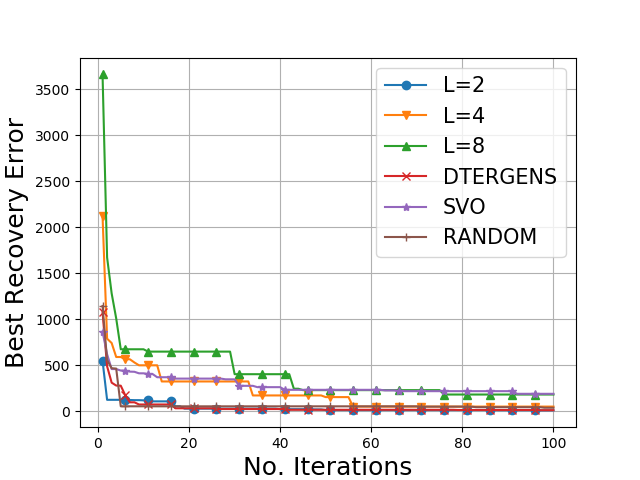
\includegraphics[width=0.45\linewidth]{./kernel_plots/synthetic_exp0.png} & 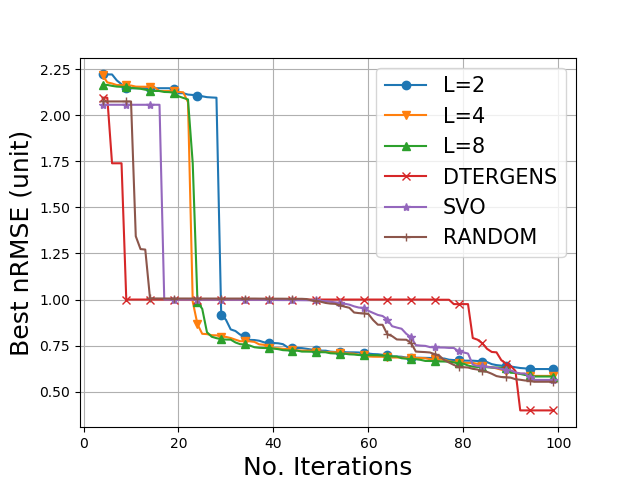
\includegraphics[width=0.45\linewidth]{./kernel_plots/diabetes.png} \\ 
\vspace{-1mm}
(L1) $\mathrm{RQ} \times \mathrm{RQ}$ & (R1) DIABETES \\
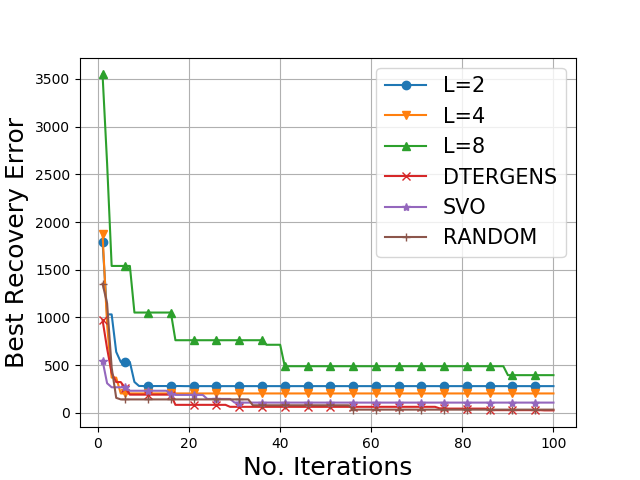
\includegraphics[width=0.45\linewidth]{./kernel_plots/synthetic_exp1.png} & 
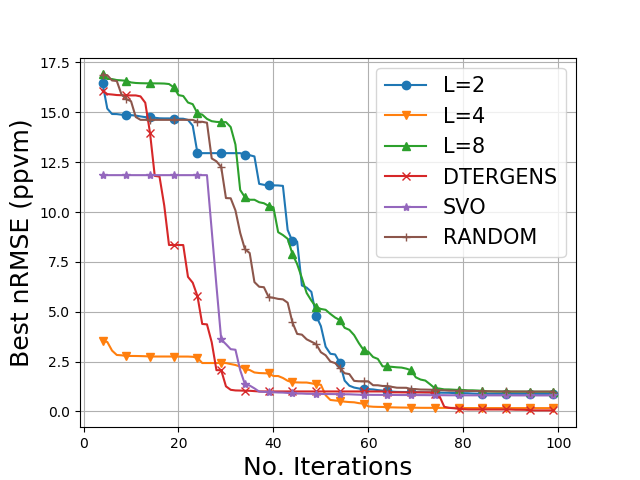
\includegraphics[width=0.45\linewidth]{./kernel_plots/mauna.png} \\ 
\vspace{-2mm}
(L2) $\mathrm{PER} \times \mathrm{RQ} \times \mathrm{LIN} \times \mathrm{LIN}$ & (R2) MAUNA LOA \\
\vspace{-3mm}
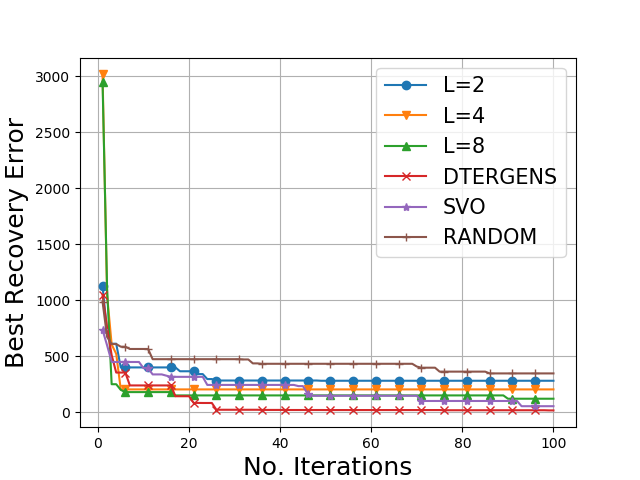
\includegraphics[width=0.45\linewidth]{./kernel_plots/synthetic_exp2.png} &
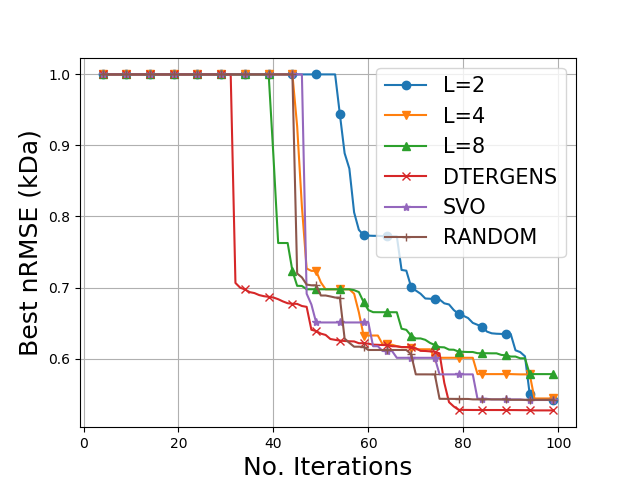
\includegraphics[width=0.45\linewidth]{./kernel_plots/protein.png} \\
\vspace{-3mm}
(L3) $\mathrm{LIN} \times \mathrm{RQ} \times \mathrm{LIN} \ + $ & (R3) PROTEIN \\
$\mathrm{PER} \times \mathrm{LIN} + \mathrm{RQ} \times \mathrm{SE}$ & \\
\end{tabular}
\caption{
(Left): Best kernel recovery error over 100 iterations with various kernel selection methods on three synthetic datasets constructed from specific kernels; (Right):
Best nRMSE over 100 iterations with various kernel selection methods on 3 benchmark datasets using vDTC~\cite{Hensman13}.}
\label{app-ks-fig:recovery}
\end{figure}
We first investigate how well various kernel selection methods recover a covariance matrix given synthetic data randomly drawn from its corresponding distribution. Unlike most real-world settings where a ground truth kernel is not known and performance evaluation relies on possibly noisy predictive accuracy, this scenario provides a ground truth for kernel selection and allows us to directly measure the success of various contending methods.

Explicitly, given an arbitrarily chosen kernel $k^{\ast}$ (with arbitrarily initialized hyper-parameters) and $n$ i.i.d. input observations $\tau = \{\mathbf{x}_1, \mathbf{x}_2 \dots \mathbf{x}_n\} \subset \mathbb{R}^d$ drawn from $\mathcal{N}(\mathbf{0}, \mathbf{I})$, we subsequently generate corresponding output observations $Y = \{y_1, y_2 \dots y_n\}$, where $y_i \sim \mathcal{N}(0, K^{\ast}_\tau + \sigma^2\mathbf{I})$ and $K^{\ast}_\tau$ denotes the data covariance matrix induced by $k^{\ast}$. We then apply various kernel selection methods, including $\textsc{DTerGenS}$ for vDTC prediction on this synthetic dataset and measure our recovery error for any selected kernel $k$ by $\mathcal{L}_{\mathrm{rec}}(k) = \|K_\tau - K^{\ast}_\tau\|_{\mathrm{Fro}}$. Fig.~\ref{app-ks-fig:recovery} (left) shows the best recovery errors achieved over a span of 100 BO iterations with 3 different ground truth kernels: (1) $k^\ast = k_\mathrm{RQ}\times k_\mathrm{RQ}$; (2) $k^\ast = k_\mathrm{PER}\times k_\mathrm{RQ}\times k_\mathrm{LIN}\times k_\mathrm{LIN}$; and (3) $k^\ast = k_\mathrm{LIN}\times k_\mathrm{RQ}\times k_\mathrm{LIN} + k_\mathrm{PER}\times k_\mathrm{LIN} + k_\mathrm{RQ}\times k_\mathrm{SE}$. 
\begin{figure}
\begin{tabular}{cc}
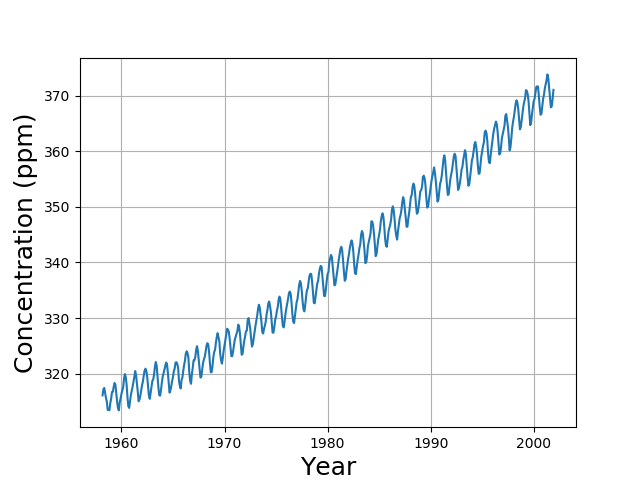
\includegraphics[width=0.48\columnwidth]{./kernel_plots/mauna_visual.png} & 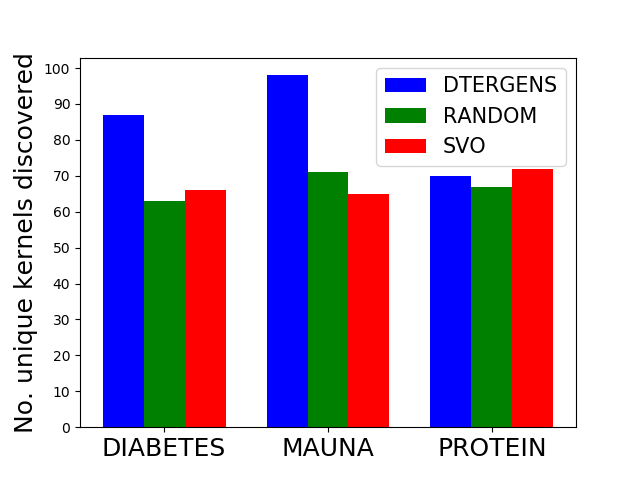
\includegraphics[width=0.48\columnwidth]{./kernel_plots/unique_k.png} \\
(a) & (b)
\end{tabular}
\caption{(a) The linear-periodic trend of the MAUNA dataset; and (b) number of unique kernels discovered by \textsc{DTerGenS}, \textsc{SVO} and random search on all three datasets.}
\label{app-ks-fig:visual}
\end{figure}

In all experiments, $\textsc{DTerGenS}$ consistently achieves the lowest recovery error after 100 iterations compared to other methods. Random search performs competitively when the ground truth kernels are simple (i.e., $L=2,4$), hence easy to be found via randomization. On the other hadn, random search expectedly performs the worst when the ground truth kernel is longer (i.e., $L=7$). We also observe that without the termination policy component, the performance of $\textsc{DTerGenS}$ is only competitive when $L$ is set to be roughly the length of the ground truth kernel, but otherwise outperformed by other methods. This shows the importance of adaptively learning the complexity of the kernel expression using a data driven policy. Lastly, we observe that $\textsc{SVO}$ is most significantly outperformed by $\textsc{DTerGenS}$ in the first
experiment. We reason that this is because the number of length-$2$ kernels is relatively smaller in the set of training expressions for the VAE component of $\textsc{SVO}$. Thus, the trained VAE could be biased to produce longer kernels and it is more difficult for $\textsc{SVO}$ to find a latent embedding that decodes to a length-$2$ kernel. In contrast, $\textsc{DTerGenS}$ does not incur this problem because its termination policy is also learned as it collects information about the embedding space.
\subsection{Kernel Selection for Regression Task}
This section investigates the performance of kernel selection for regression tasks using vDTC~\cite{Hensman13} on DIABETES~\cite{UCI_diabetes_data}, MAUNA~\cite{mauna_loa_data} and PROTEIN~\cite{UCI_protein_data} datasets. In all experiments, we measure performance by computing the root-mean-square-error of predictions, normalized against the root-mean-square-error achieved by fixing the kernel of \textsc{vDTC} to be $k_{\mathrm{SE}}$, which serves to demonstrate the improvement over the default choice of kernel. Explicitly, our kernel selection metric for any selected kernel $k$ is given by:
\begin{eqnarray}
\mathrm{nRMSE}(k) &\triangleq& \sqrt{\frac{\sum_{i=1}^{n_{\mathrm{test}}} \left(\bar{y}_i(k) - y_i\right)^2 }{\sum_{i=1}^{n_{\mathrm{test}}} \left(\bar{y}_i(k_{SE}) - y_i\right)^2}}
\end{eqnarray}
where $\bar{y}_i(k)$ denotes the prediction made by vDTC for test input $\mathbf{x}_i$ with selected kernel function $k$ and $y_i$ denotes the corresponding ground truth test output. 

Fig.~\ref{app-ks-fig:recovery} (right) shows the comparative performance between $\textsc{DTerGenS}$ and the competing methods. Across all datasets, $\textsc{DTerGenS}$ consistently obtains the best performing kernel expression. On the PROTEIN dataset, $\textsc{DTerGenS}$ also shows the fastest convergence among all competing methods. On the MAUNA dataset, $\textsc{DTerGenS}$ performs competitively with $L=4$ and both variants of $\textsc{DTerGenS}$ outperform $\textsc{SVO}$. More interestingly, the best kernel found for the MAUNA dataset is $k_\mathrm{LIN}\times k_\mathrm{PER}\times k_\mathrm{PER} + k_\mathrm{RQ}\times k_\mathrm{PER}$, which accurately reflects the linearly increasing periodic nature of the data (Fig.~\ref{app-ks-fig:visual}a).

Fig.~\ref{app-ks-fig:visual}b further compares the expressiveness of the three kernel selection methods (i.e., \textsc{DTerGenS}, \textsc{SVO} and random search), which is measured by the number of unique kernels found over 100 iterations in each method. As expected, random search consistently produces the same amount of unique expressions across all experiments. While $\textsc{SVO}$ discovers approximately the same amount of unique kernels as does random search on all three datasets, it tends to outperform random search as its discovery is guided. Finally, we observe that $\textsc{DTerGenS}$ consistently discovers more unique kernels and also outperforms the other methods. This finding asserts our earlier intuition on how adding expressiveness to the embedding method also helps to improve search efficiency.